% Options for packages loaded elsewhere
\PassOptionsToPackage{unicode}{hyperref}
\PassOptionsToPackage{hyphens}{url}
%
\documentclass[
]{article}
\usepackage{lmodern}
\usepackage{amssymb,amsmath}
\usepackage{ifxetex,ifluatex}
\ifnum 0\ifxetex 1\fi\ifluatex 1\fi=0 % if pdftex
  \usepackage[T1]{fontenc}
  \usepackage[utf8]{inputenc}
  \usepackage{textcomp} % provide euro and other symbols
\else % if luatex or xetex
  \usepackage{unicode-math}
  \defaultfontfeatures{Scale=MatchLowercase}
  \defaultfontfeatures[\rmfamily]{Ligatures=TeX,Scale=1}
\fi
% Use upquote if available, for straight quotes in verbatim environments
\IfFileExists{upquote.sty}{\usepackage{upquote}}{}
\IfFileExists{microtype.sty}{% use microtype if available
  \usepackage[]{microtype}
  \UseMicrotypeSet[protrusion]{basicmath} % disable protrusion for tt fonts
}{}
\makeatletter
\@ifundefined{KOMAClassName}{% if non-KOMA class
  \IfFileExists{parskip.sty}{%
    \usepackage{parskip}
  }{% else
    \setlength{\parindent}{0pt}
    \setlength{\parskip}{6pt plus 2pt minus 1pt}}
}{% if KOMA class
  \KOMAoptions{parskip=half}}
\makeatother
\usepackage{xcolor}
\IfFileExists{xurl.sty}{\usepackage{xurl}}{} % add URL line breaks if available
\IfFileExists{bookmark.sty}{\usepackage{bookmark}}{\usepackage{hyperref}}
\hypersetup{
  pdftitle={Annual Report 2021},
  hidelinks,
  pdfcreator={LaTeX via pandoc}}
\urlstyle{same} % disable monospaced font for URLs
\usepackage[margin=1in]{geometry}
\usepackage{graphicx,grffile}
\makeatletter
\def\maxwidth{\ifdim\Gin@nat@width>\linewidth\linewidth\else\Gin@nat@width\fi}
\def\maxheight{\ifdim\Gin@nat@height>\textheight\textheight\else\Gin@nat@height\fi}
\makeatother
% Scale images if necessary, so that they will not overflow the page
% margins by default, and it is still possible to overwrite the defaults
% using explicit options in \includegraphics[width, height, ...]{}
\setkeys{Gin}{width=\maxwidth,height=\maxheight,keepaspectratio}
% Set default figure placement to htbp
\makeatletter
\def\fps@figure{htbp}
\makeatother
\setlength{\emergencystretch}{3em} % prevent overfull lines
\providecommand{\tightlist}{%
  \setlength{\itemsep}{0pt}\setlength{\parskip}{0pt}}
\setcounter{secnumdepth}{-\maxdimen} % remove section numbering
\usepackage{amsmath}
\usepackage{booktabs}
\usepackage{caption}
\usepackage{longtable}

\title{Annual Report 2021}
\author{}
\date{\vspace{-2.5em}}

\begin{document}
\maketitle

\hypertarget{purpose}{%
\section{Purpose}\label{purpose}}

Oral reading fluency (ORF), generally defined as reading quickly,
accurately, and with prosody, is an essential part of reading
proficiency. Prosody, reading with appropriate expression and phrasing,
is one way to demonstrate that a reader understands the meaning of the
text.

The purpose of this study is to collect prosody ratings of audio
recordings of students' ORF. These human-rated prosody scores will serve
as the basis for training an algorithm that can be used to automatically
generate prosody scores from students' oral reading.

\hypertarget{audio-recordings}{%
\section{Audio Recordings}\label{audio-recordings}}

Audio recordings of students in Grades 2 through 4 reading brief ORF
passages were collected as part of an
\href{https://ies.ed.gov/funding/grantsearch/details.asp?ID=1492}{IES
funded project} called Computerized Oral Reading Evaluation, or
\href{https://jnese.github.io/core-blog/}{CORE}. CORE combines automatic
speech recognition (ASR) to score ORF accuracy and rate, with a latent
variable psychometric model to scale, equate, and link scores across
Grades 2 through 4. The primary goal of CORE is to develop an ORF
assessment system with the potential to reduce: (a) human ORF
administration errors, by standardizing administration setting,
delivery, and scoring; (b) the time cost of ORF administration, by
allowing small-group or whole-classroom testing; (c) the resource cost
to train staff to administer and score the ORF assessment; and (d) the
standard error of ORF measurement.

The work conducted in the
\href{https://ies.ed.gov/funding/grantsearch/details.asp?ID=3427}{current
project} extends this line of research by incorporating prosody into the
measurement model.

The
\href{https://jnese.github.io/core-blog/posts/2019-04-12-consequential-validity-study-procedures/}{Consequential
Validity Study} from the original CORE project conducted in 2017-18 and
2018-19 resulted in the accumulation of 90,720 audio files. Of these,
8,713 were excluded from the current study because they were recordings
of students reading the criterion easyCBM ORF passages from the original
study while the remaining 82,007 (90.4\%) represented recordings of
students reading brief (approximately 50-85 word) passages developed
specifically for the CORE project. From the 82,007 eligible audio
recordings, only those that were at least ten seconds long were selected
(to screen for empty or incomplete files) for a final corpus of 78,712
audio files.

\hypertarget{core-orf-passages}{%
\subsection{CORE ORF Passages}\label{core-orf-passages}}

CORE passages were written by a former teacher, who also co-wrote the
original easyCBM ORF and reading comprehension passages. Each CORE
passage is an original work of fiction, and within 5 words of a targeted
length: \emph{long} = 85 words or \emph{medium} = 50 words. Each passage
has a beginning, middle, and end, follows either a
``problem/resolution'' or ``sequence of events'' format, and contains
minimal use of dialogue and symbols. Exclusion rules for what could not
appear in passages included: religious themes; trademark names, places,
products; cultural/ethnic depictions; age-inappropriate themes (e.g.,
violence, guns, tobacco, drugs). All final CORE passages were reviewed
by two experts in assessment for screening and progress monitoring for
errors (e.g., format and grammatical), and bias (e.g., gender, cultural,
religious, geographical). Final passages included 150 total passages, 50
at each of Grades 2-4, with 20 long passages (80-90 words), and 30
medium passages (45-55 words) for each grade.

\hypertarget{audio-file-selection}{%
\subsection{Audio File Selection}\label{audio-file-selection}}

For the current study, a two-step process was used to select 200 audio
files for 10 CORE ORF passages at each of Grades 2 through 4.

First, for each grade and passage length the 5 CORE passages with the
greatest number of audio file records were selected to create as large
an item bank as possible. This process resulted in the selection of 10
CORE passages (5 long and 5 medium) for each of Grades 2 -- 4, 30
passages in all.

Second, stratified random sampling was applied to select 200 audio
recordings of each CORE passage, oversampling for English learners (ELs)
and students with disabilities (SWDs), two student groups for which the
ASR may be less accurate. Of the 1388 students in the full sample,
approximately \% were dually classified as EL and SWD, \% were
classified as EL only, \% were classified as SWD only, \% were
classified as neither EL nor SWD.

The stratified random sampling plan led to the following quantities of
sampled audio files: 5 students (2.5\%) dually classified as EL and SWD,
65 students (32.5\%) classified as EL only, 65 students (32.5\%)
classified as SWD only, and 65 students (32.5\%) classified as neither
EL nor SWD. A cascading logic was implemented, such that when fewer than
5 recordings included students dually classified as EL and SWD, the
remainder of recordings was sampled from students classified as EL only.
If there were insufficient audio recordings from EL only students, the
remainder was sampled from students classified as SWD only. The
remainder of audio recordings was sampled from students classified as
neither EL nor SWD, of which there were ample recordings.

The design of the project stipulated that each of the 200 audio files
per CORE passage was to be rated for prosody by two different raters,
for a total of 12,000 prosody ratings (10 passages * 3 grade levels *
200 recordings * 2 ratings = 12,000 total prosody ratings).

The 6,000 audio files were grouped into 120 sets of 50 for distribution
to human raters. The 200 audio files per CORE passage were split into
four sets, such that each set of 50 contained audio files of students
reading the same passage. This structure was used to allow raters to get
familiar with a passage and thus provide more reliable ratings. The PI
(J. F. T. Nese) manually distributed the sets as required, descending by
grade and passage such that all four sets of the first Grade 4 passage
were sent to the first eight raters (as each set was rated twice), and
continuing through the last Grade 2 passage.

\begin{verbatim}
## Warning in mask$eval_all_mutate(quo): NAs introduced by coercion
\end{verbatim}

Of the 6,000 selected audio files 836 (14\%) had to be replaced because
they had no audio available to score; either there was no audio (e.g.,
the student was muted or advanced without reading), or the audio did not
allow the rater to confidently give a prosody score (e.g., poor audio
quality, too much background noise, a very quiet reader). All audio
files were replaced with a reading from the same CORE passage. For
\emph{n} audio files that needed to be replaced for a CORE passage,
\emph{n} \(\times\) 1.175 (17.5\% of \emph{n}) were sampled to account
for potential audio recording with no available audio in the replacement
set. An effort was made to replace audio files read by a student with
the same EL/SWD classification. That is, the same cascading logic as
previously described was applied, such that when the number of
recordings for students dually classified as EL and SWD was less than
required in our sampling plan, the remainder was sampled from students
classified as EL only. If there were insufficient audio recordings from
EL only students, the remainder was sampled from students classified as
SWD only. Insufficient recordings led to the remainder of audio
recordings being sampled from students classified as neither EL nor SWD,
of which there were ample recordings. An additional 998 audio files were
distributed to the human raters as replacements.

After the 998 audio file replacements were scored, there remained five
CORE passages that had less than 200 audio files with two different
prosody ratings: three CORE passages had 199 audio files, and two had
197 audio files. For \emph{n} (1 or 3) audio files that needed to be
replaced for a CORE passage, \emph{n} \(\times\) 7 were sampled to
account for potential audio recording with no available audio in the
replacement set. These audio files were randomly sampled (without
stratifying for ELs and SWDs) from those remaining for the respective
CORE passages.

After all selected and usable audio files were rated twice, the final
sample included 14,122 audio files from 1,388 students (4,900 in Grade
2, 4,650 in Grade 3, 4,572 in Grade 4). The number of audio files per
student in the final sample ranged from 2 to 44.

The results of the stratification yielded a sample of 14,122 audio files
that was 3\% (\emph{n} = 358) EL and SWD, 24\% (\emph{n} = 3414) EL
only, 30\% (\emph{n} = 4208) SWD only, and 43\% (\emph{n} = 6142)
neither EL or SWD.

\begin{verbatim}
## Warning: The `.dots` argument of `group_by()` is deprecated as of dplyr 1.0.0.
\end{verbatim}

\captionsetup[table]{labelformat=empty,skip=1pt}
\begin{longtable}{lcc}
\caption*{
\large Sample Demographic Characteristics\\ 
} \\ 
\toprule
& & & \\ 
 
\textbf{Characteristic} & \textbf{N = 1,388}\textsuperscript{1} & \textbf{N = 14,122}\textsuperscript{1} \\ 
\midrule
Grade &  &  \\ 
2 & 485 (35\%) & 4,900 (35\%) \\ 
3 & 450 (32\%) & 4,650 (33\%) \\ 
4 & 453 (33\%) & 4,572 (32\%) \\ 
Gender &  &  \\ 
Female & 609 (49\%) & 5,646 (45\%) \\ 
Male & 643 (51\%) & 6,930 (55\%) \\ 
(Missing) & 136 & 1,546 \\ 
Ethnicity &  &  \\ 
Hispanic/Latino & 327 (26\%) & 4,188 (33\%) \\ 
Not Hispanic/Latino & 925 (74\%) & 8,388 (67\%) \\ 
(Missing) & 136 & 1,546 \\ 
Race &  &  \\ 
American Indian/Native Alaskan & 52 (4.2\%) & 658 (5.2\%) \\ 
Asian & 9 (0.7\%) & 130 (1.0\%) \\ 
Black/African American & 5 (0.4\%) & 56 (0.4\%) \\ 
Hispanic & 45 (3.6\%) & 354 (2.8\%) \\ 
Multi-Racial & 108 (8.6\%) & 1,030 (8.2\%) \\ 
Native Hawaiian/Other Pacific Islander & 4 (0.3\%) & 48 (0.4\%) \\ 
White & 1,029 (82\%) & 10,300 (82\%) \\ 
(Missing) & 136 & 1,546 \\ 
Students with Disabilities (SWD) & 242 (17\%) & 4,566 (32\%) \\ 
English Language Learners (EL) & 197 (14\%) & 3,772 (27\%) \\ 
Stratification Groups &  &  \\ 
EL \& SWD & 23 (1.7\%) & 358 (2.5\%) \\ 
EL only & 174 (13\%) & 3,414 (24\%) \\ 
Not EL or SWD & 972 (70\%) & 6,142 (43\%) \\ 
SWD only & 219 (16\%) & 4,208 (30\%) \\ 
\bottomrule
\end{longtable}
\vspace{-5mm}
\begin{minipage}{\linewidth}
\textsuperscript{1}n (\%) \\ 
\end{minipage}

\hypertarget{research-team}{%
\section{Research Team}\label{research-team}}

The
\href{https://jnese.github.io/coreprosody/research_team.html}{research
team} comprised four faculty with expertise in the assessment of
students' reading fluency (specializations included: two doctorates in
School Psychology, one doctorate in Educational Leadership with a
specialization in Learning Assessment/Systems Performance, and one
doctorate in Educational Psychology), and one graduate research
assistant with experience in literacy. The research team met weekly from
August through November 2020, to refine a prosody scoring rubric, score
audio files to be used as training and demonstration exemplars, and
develop two online sessions to train prosody raters. These sessions were
delivered live as well as recorded for asynchronous delivery for raters
who were unable to attend in person.

\hypertarget{prosody-rubric-development}{%
\section{Prosody Rubric Development}\label{prosody-rubric-development}}

The research team began with the prosody scoring rubric developed by the
National Assessment of Educational Progress (NAEP; \footnote{\href{https://nces.ed.gov/nationsreportcard/pdf/studies/2006469.pdf}{Daane
  et al., 2005}}), a four-point scale (below) that focuses on phrasing,
adherence to the author's syntax, and expressiveness to assess prosody
at Grade 4.

\begin{figure}
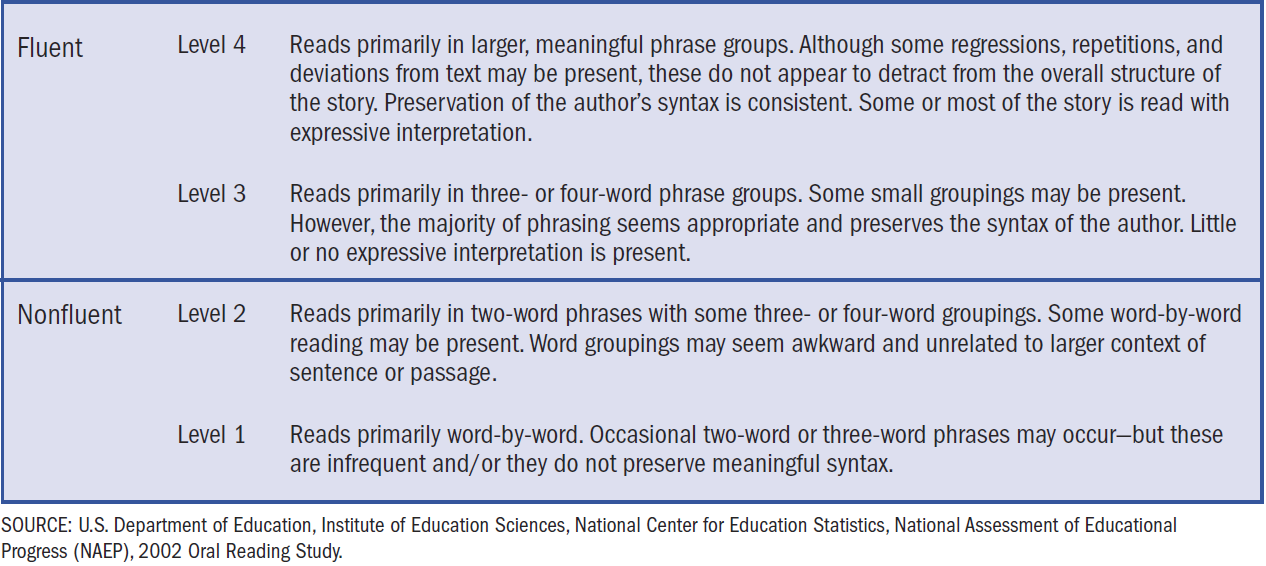
\includegraphics[width=17.58in]{C:/Users/jnese/Desktop/BRT/GRANT-CORE_II/project/coreprosody/docs/images/naep_rubric} \caption{From [Daane, Campbell, Grigg, Goodman, & Oranje (2005)](https://nces.ed.gov/nationsreportcard/pdf/studies/2006469.pdf)}\label{fig:unnamed-chunk-1}
\end{figure}

Although NAEP only applied the scoring rubric to Grade 4, our research
team made the decision to use the rubric across Grades 2 through 4,
independent of grade and based on the absolute prosody criteria
specified for each of the four prosody levels.

To help draw clear differences between the four prosody levels across
grades, parts of the Multi-Dimensional Fluency Scoring Guide (MFSG;
\footnote{\href{https://www.tandfonline.com/doi/pdf/10.1080/19388070802468715}{Rasinski
  et al., 2009}}) were incorporated into the original NAEP rubric.

\begin{figure}
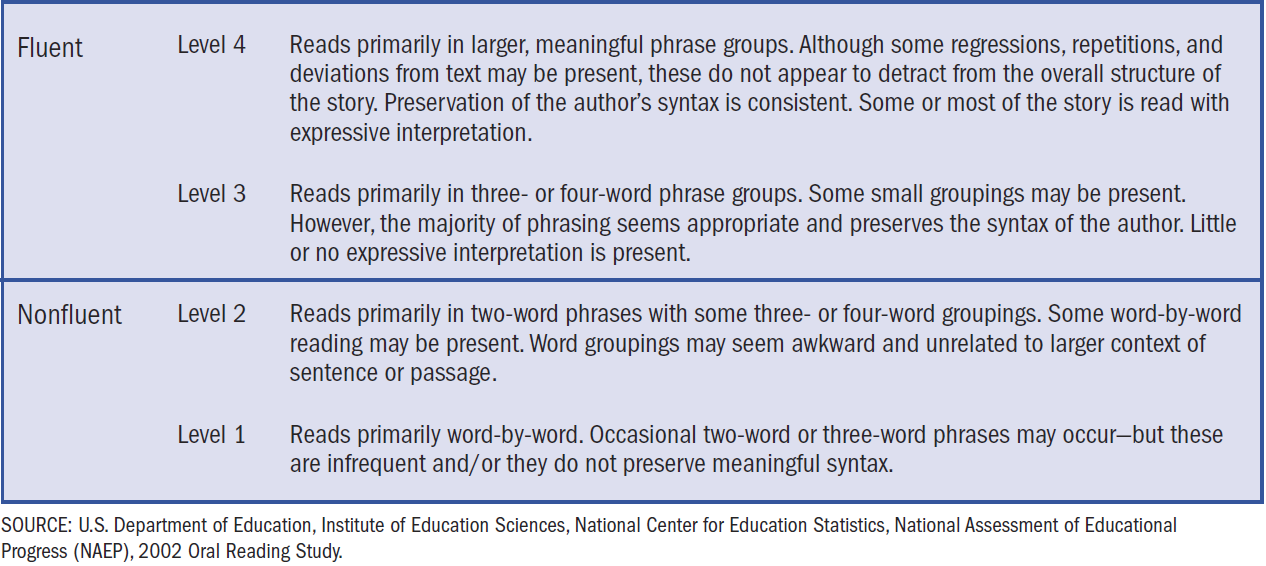
\includegraphics[width=17.58in]{C:/Users/jnese/Desktop/BRT/GRANT-CORE_II/project/coreprosody/docs/images/naep_rubric} \caption{From [Rasinski, Rikli, & Johnston (2009)](https://www.tandfonline.com/doi/pdf/10.1080/19388070802468715)}\label{fig:unnamed-chunk-2}
\end{figure}

The MFSG focuses on assessing aspects of expression, phrasing,
smoothness, pacing, and accuracy. The research team expanded and refined
the NAEP prosody rubric with select parts of the MFSG to add more
specific language and examples.

A systematic process for adapting the NAEP rubric was conducted in
August and September, 2020. First, 30 audio recordings were dispersed
among the research team and scored individually by the four faculty.
These scores and commentary were documented, analyzed, and discussed
during the following week's meetings. A summary of the team's individual
scores was presented, highlighting areas of agreement and disagreement:
9 audio files (30\%) received the same score across all four raters; 13
(43\%) received the same score across three raters with the fourth
rating different by one prosody level; 4 (13\%) were split down the
middle, with two sets of identical scores that differed by one prosody
level; and 4 (13\%) received three different prosody scores, two of
which were scored the same and two of which differed by two prosody
levels. Based on inconsistent variation within the team, it was decided
that more in-depth explanation was needed for each of the score levels.

To achieve this goal, the team listened to recordings together during
online meetings and iteratively specified deeper distinctions between
adjacent scores using the MFSG factors of pace, phrasing, and expression
and volume. The 30 audio recordings were again scored individually by
the four faculty: 12 (40\%) audio files (30\%) received the same score
across all four raters; 12 (40\%) received the same score across three
raters, with the fourth rating different by one prosody level; and 6
(20\%) were split down the middle, with two sets of identical scores
that differed by one prosody level.

The team further refined the adapted rubric to clarify rating criteria
and arrive at more unequivocal prosody scores. That is, the first
version of the adapted rubric did not address whether the overall
storyline was ``represented'' by the reader. After working through
various examples, the research team added the following distinctions for
each proficiency level (italic text represents additions from the MFSG,
and regular text represents additions made by the research team).

\begin{itemize}
\tightlist
\item
  \textbf{Level 1}: \emph{Reads slowly and laboriously.} Story line is
  incoherent.
\item
  \textbf{Level 2}: \emph{Reads moderately slowly.} Overall meaning of
  the text is preserved.
\item
  \textbf{Level 3}: \emph{Reads with a mixture of run-ons, mid-sentence
  pauses for breath, and some choppiness. There is reasonable stress and
  intonation.}
\item
  \textbf{Level 4}: \emph{Reads smoothly with some breaks, but
  self-corrects with difficult words and/or sentence structures. Reads
  with varied volume and expression (like talking to a friend with voice
  matching the interpretation of the passage).}
\end{itemize}

\hypertarget{the-core-prosody-rubric}{%
\subsection{The CORE + Prosody Rubric}\label{the-core-prosody-rubric}}

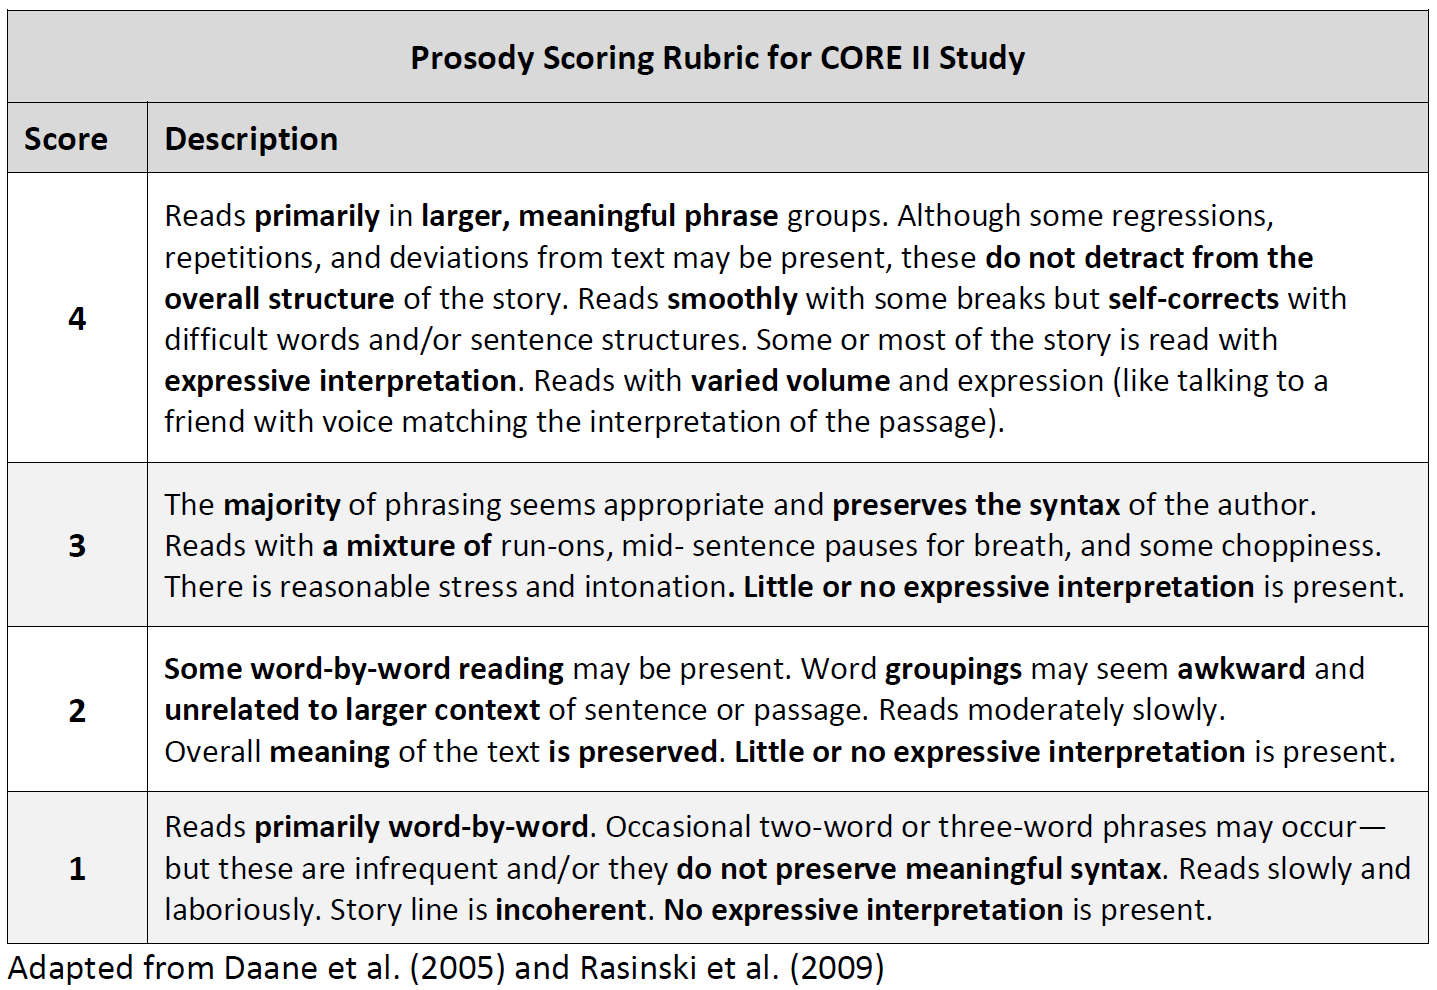
\includegraphics[width=19.96in]{C:/Users/jnese/Desktop/BRT/GRANT-CORE_II/project/coreprosody/docs/images/core-ii_rubric}

\hypertarget{exemplar-audio-files}{%
\subsection{Exemplar Audio Files}\label{exemplar-audio-files}}

After finalizing the refined rubric, the research team came to unanimous
agreement on the 30 audio files. Then, additional audio files were
sought with the goal of having 15 exemplar audio files for each of the
four prosody levels. ORF data from the CORE project were used to find
(de-identified) students whose fall easyCBM ORF scores clustered around
a specified percentile; for example, students who scored at or below the
20th percentile as potential candidates for prosody scores of Levels 1
or 2, and students who scored above the 90th percentile as potential
candidates for a prosody score of Level 4. Using this process, the team
identified an additional 31 audio files, each of which were
independently scored by two of the five research team personnel. Of
these, 21 (68\%) received the same score across the two raters. The
remaining 10 audio files were scored by a third member of the research
team, and discussed by the full research team until unanimous score
agreement was achieved. Additional exemplar audio files were still
needed for Levels 2 and 4, so 16 additional files were identified and
underwent the same process just described.

In total, 81 passages were identified and scored by the research team as
exemplars for trainings and demonstrations: 20 at Level 4, 23 at Level
3, 15 at Level 2, and 23 at Level 1. Of these, 24 were used for
Training, 25 were used for Certification (both described below), and the
remaining 32 were retained in case of future need.

Human prosody raters were recruited and required to complete two
\href{https://jnese.github.io/coreprosody/human_prosody_scoring.html\#training-development-implementation}{Training
Sessions}, and meet
\href{https://jnese.github.io/coreprosody/human_prosody_scoring.html\#prosody-certification}{Prosody
Certification} criterion.

\hypertarget{prosody-rater-recruitment}{%
\section{Prosody Rater Recruitment}\label{prosody-rater-recruitment}}

Educators (teachers and specialized professionals) were targeted as
potential prosody raters. Potential prosody raters were recruited in
October -- November 2020 from two sources: teacher participants from the
original CORE project, and through an announcement placed on the easyCBM
- Lite and Deluxe sites for three weeks (10/19/2020 -- 11/6/2020). These
two easyCBM sites have over 79,000 registered users.

\begin{quote}
Paid Opportunity! * We're looking for Grade 2-5 teachers interested in
earning a little extra money scoring oral reading for prosody
(expressiveness). * All work can be done remotely on your own time. * No
prior experience scoring prosody needed (we'll provide the training). *
The more readings you score, the more money you will earn! * This
project is part of an IES-funded research study to develop
computer-scored oral reading fluency measures. * For more information,
please email: ------@easycbm.com
\end{quote}

Approximately 300 people responded to the announcement posted on the
easyCBM sites. These respondents were then sent an email introducing
them to the project, the task required of them, what they could expect
(payment terms, remote work, and work commitment), training
requirements, the prosody certification process, and next steps (a
Qualtrics Registration form requiring demographic information, teaching
experience, and a W9). The PI (J. F. T. Nese) corresponded with all
potential prosody raters throughout the process.

\begin{quote}
Thank you for expressing interest in the CORE II Prosody Study! My name
is Joe Nese, I am an education researcher at the University of Oregon,
and I am leading the project.
\end{quote}

\begin{quote}
\textbf{Task:} For this project, we have thousands of audio files from
students in Grades 2-4, reading very short passages (less than 90
seconds each). We need educators (you!) to listen to these audio files
and rate them for prosody -- the expressiveness with which the student
read the passage. These scores will serve as the basis for our
subsequent study to automatically generate prosody scores, which will
provide teachers with important information about their students'
reading. All of the audio files were collected in a previous research
study.
\end{quote}

\begin{quote}
\textbf{What to expect:} You will be paid \$1.25 for every passage you
rate. Each passage is no more than 90 seconds in length, and we expect
you will listen to a passage 2-3 times before you submit your rating.
You can make up to \$25 per hour if you are working carefully and
efficiently. Payment will not be processed until all work is complete
(i.e., all audio files are scored), but no later than April 30, 2021.
\end{quote}

\begin{quote}
You will work remotely, from your computer! We have an online system so
that you can log in and listen to and score the audio files assigned to
you. The work will start in November and continue until all audio files
are scored. This could take several weeks, or several months, depending
on how quickly everyone works. Regardless, you can work on your own
time. But we ask that if you sign up, you commit to scoring at least 100
audio files (approximately 5-7 hours of work). You must score at least
50 passages before any payment will be remitted.
\end{quote}

\begin{quote}
\textbf{Before you begin:} Before you start, you will need to attend two
trainings (about 3-4 hours, total), where we will teach you everything
you need for this project. You will be paid \$15/hour for the training
sessions. You will also need to demonstrate proficiency in rating
prosody by scoring 80\% or higher on two different sets of audio files
which have previously been scored by the research team. If you do not
meet the criteria, you will not be eligible to participate in the
project (but you will be paid for attending the trainings, of course).
\end{quote}

\begin{quote}
We have scheduled two dates for each of the two required trainings
sessions. You may choose either of the two dates listed for each
training, but you must attend both Training Session \#1 and Training
Session \#2. * Training Session \#1: Nov 13 or Nov 16 3:30-5:30 Pacific
* Training Session \#2: Nov 20 or Nov 23 3:30-5:00 Pacific
\end{quote}

\begin{quote}
If you are interested in participating in this project, please click the
link below to enroll! You will answer some questions about yourself,
sign up for training dates, and importantly, submit a W9 so that you can
be paid for your work. You cannot join the project without completing
and submitting the W9. The blank W9 is embedded in the survey, and also
attached here. It will likely be easier to complete the attached W9
before you start the survey so that it is ready to upload.
\end{quote}

\begin{quote}
Click the link below to sign-up!
\end{quote}

\begin{quote}
Thank you so much for your interest in partnering with us on this
important work. We are grateful for all you do on behalf of children.
\end{quote}

Of the 300 respondents, 119 completed the Registration form, and 78
completed the required trainings. (No information is available as to why
some chose not to complete the Registration or the trainings.)

\hypertarget{prosody-certification}{%
\section{Prosody Certification}\label{prosody-certification}}

Prior to starting work, each prosody rater was required to complete the
Training and demonstrate scoring proficiency by obtaining 80\% or higher
agreement with the research team's pre-determined rating on two
different sets of five audio files. Raters had five opportunities to
achieve at least 80\% (4/5) on two of the prosody assessments. Raters
unable to achieve two passing scores received payment for their
participation in training (\$45) but were not be eligible to continue
their participation in this project.

All Prosody Certification Assessments were delivered with Google Forms'
Quiz feature. All participants took the first Prosody Certification
after Training \#1 and before Training \#2. The remaining Prosody
Certification assessments were taken at each participant's pace. Once a
participant met the prosody certification criteria by scoring at least
80\% on two assessments, they began scoring audio files (and took no
more assessments).

Of the 78 people who completed the
\href{https://jnese.github.io/coreprosody/human_prosody_scoring.html\#training-development-implementation}{Trainings},
63 (81\%) met prosody certification, 2 (3\%) failed to meet
certification, and 13 (17\%) did not complete the certification process.

\captionsetup[table]{labelformat=empty,skip=1pt}
\begin{longtable}{lcclcl}
\caption*{
\large Prosody Certification Assessment Passing Rates\\ 
} \\ 
\toprule
 & n & Fail & Fail (\%) & Pass & Pass (\%) \\ 
\midrule
Certification \#1 & 78 & 37 & 47\% & 41 & 53\% \\ 
Certification \#2 & 73 & 20 & 27\% & 53 & 73\% \\ 
Certification \#3 & 41 & 6 & 15\% & 35 & 85\% \\ 
Certification \#4 & 10 & 5 & 50\% & 5 & 50\% \\ 
Certification \#5 & 4 & 1 & 25\% & 3 & 75\% \\ 
\bottomrule
\end{longtable}

Of the 78 people who took Certification \#1, 53\% passed by scoring 4 or
5; 73\% of the 73 people who took Certification \#2 passed; 85\% of the
41 people who took Certification \#3 passed; 50\% of the 10 people who
took Certification \#4 passed; and 75\% of the 4 people who took
Certification \#5 passed.

\begin{verbatim}
## Warning: Removed 4 rows containing missing values (position_stack).
\end{verbatim}

\begin{verbatim}
## Warning: Removed 4 rows containing missing values (geom_text).
\end{verbatim}

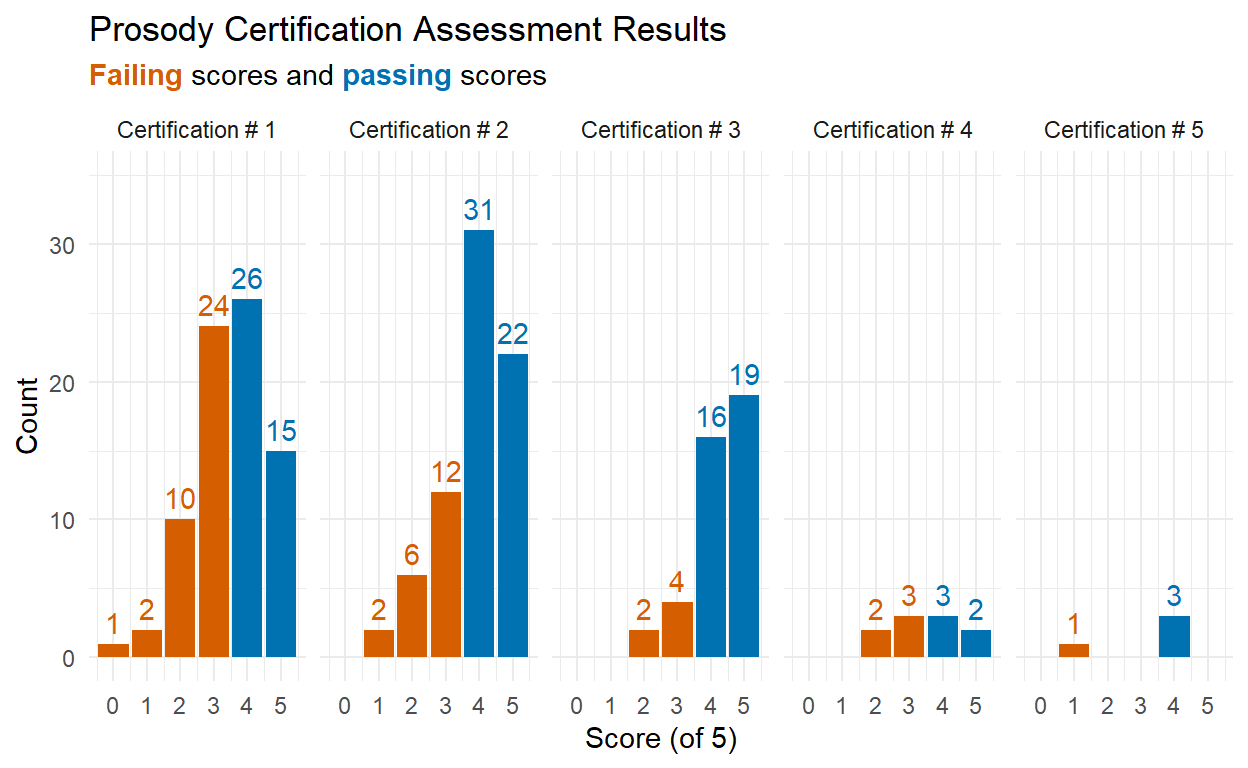
\includegraphics{annual_report_2021_files/figure-latex/traincert_plot-1.pdf}

\hypertarget{training-development-implementation}{%
\section{Training Development \&
Implementation}\label{training-development-implementation}}

A two-session training for prosody raters was developed for in-person,
online delivery across two meetings in November 2020. Each Training
Session was delivered twice: on Friday and the subsequent Monday
afternoon (after the school day had concluded), and participants could
attend either the Friday or the Monday training. There was one week
between Training Session \#1 and Session \#2. For Training Session \#1,
Day 1 was held on 11/13/2020 and Day 2 was held on 11/16/2020. For
Training Session \#2, Day 1 was held on 11/20/2020 and Day 2 was held on
11/23/2020.

Three members of the team were present to deliver content and answer
questions using Powerpoint slides presented on the Zoom platform for
web-based, live interaction. All trainings were recorded via Zoom for
asynchronous training for participants who could not attend one or both
of the live trainings. In total, 78 people completed the trainings.

\captionsetup[table]{labelformat=empty,skip=1pt}
\begin{longtable}{lccc}
\caption*{
\large Training Sessions Attendance\\ 
} \\ 
\toprule
Training Session & Day 1 & Day 2 & Asynchronous \\ 
\midrule
Session \#1 & 35 & 35 & 8 \\ 
Session \#2 & 34 & 35 & 9 \\ 
\bottomrule
\end{longtable}

The research team created a
\href{https://jnese.github.io/CORE-II_trainingwebsite/index.html}{website}
for participants to access training resources. The website included: the
\href{https://jnese.github.io/CORE-II_trainingwebsite/\#the-task}{seven-step
process} for scoring audio files; the
\href{https://jnese.github.io/CORE-II_trainingwebsite/prosody_rubric.html}{prosody
rubric} as a resource to print or keep open when rating;
\href{https://jnese.github.io/CORE-II_trainingwebsite/training_materials.html}{training
materials}, including the presentation slides, and a recording of each
Training Session; the 24
\href{https://jnese.github.io/CORE-II_trainingwebsite/exemplar_audiofiles.html}{exemplar
audio files} from Training Session \#1; the link to the scoring site;
and an
\href{https://ies.ed.gov/funding/grantsearch/details.asp?ID=34270}{About}
page with information about the study.

\hypertarget{training-session-1}{%
\subsection{Training Session \#1}\label{training-session-1}}

During Training Session \#1 (2 hours), study logistics and key concepts
were explained to potential raters.
\href{https://jnese.github.io/CORE-II_trainingwebsite/CORE_training_session1day2_FINAL.pdf}{Training}
included: information about the project context; a comprehensive review
of prosody; the task of rating audio recordings for prosody; an
explanation of the rubric and how to rate recordings; how to earn
certification as prosody rater; the expectations and payment structure;
a set of 12 exemplar audio files (about one recording per prosody level
for each of Grades 2 -- 4); and a practice exercise, consisting of 12
exemplar audio files (three at each of the four prosody levels presented
randomly) followed by a discussion of each and the qualities that made
it a specific prosody level.

Participants were also introduced to prosody scoring in partial
increments of 0.5 to facilitate prosody ratings in cases of nuanced
uncertainty. For example, if a rater's prosody rating was undecided
between Level 2 and 3, they could score it as a 2.5. For the purposes of
the study, all half scores (i.e., 1.5, 2.5, and 3.5) were rounded down
because they did not meet the threshold for a higher score.

The Training Session \#1 practice exercise involved three rounds of
listening to each audio file. The purpose of the first listen was to pay
attention to the passage's general meaning so that raters would have a
general sense of what the passage was about and the degree to which the
student's reading conveyed the meaning. The purpose of the second listen
was to train raters to pay attention to reading style (i.e.,
word-by-word, awkward word groups, conversational) and to notice whether
the author's syntax was preserved. The third listen was used to train
raters to pay attention to expressiveness. This step-by-step process was
designed to train raters to attend to all aspects of the rubric, and not
to focus exclusively on any single aspect. The team developed a
seven-step guide for listening to and scoring audio recordings.

\hypertarget{the-task}{%
\paragraph{The Task}\label{the-task}}

\begin{figure}
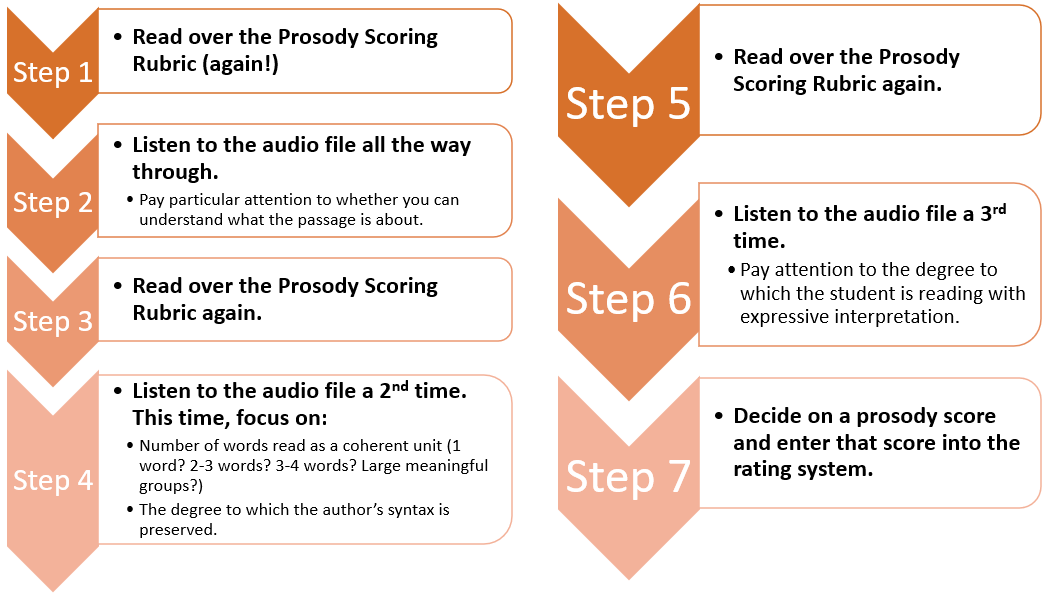
\includegraphics[width=14.53in]{C:/Users/jnese/Desktop/BRT/GRANT-CORE_II/project/coreprosody/docs/images/task_7steps} \end{figure}

After listening to example recordings to clarify the scale, participants
were able to practice on their own. Recordings were played, and
participants were asked to first think about how they would rate the
recording without sharing their scores, and then they were prompted to
type their prosody score for the recorded reading into the Zoom
platform's chat box feature. Participants' reasoning for scores was
discussed as a large group with research team members facilitating the
discussion and using the rubric to emphasize points made.

After Training Session \#1, participants were given the first Prosody
Certification assessment, which consisted of five audio files to be
scored individually, on their own time, before Training Session \#2 .

Of the 78 people who took the Prosody Certification Assessment \#1, 41
(53\%) passed and 37 (47\%) did not. Note that Certification \#1 was
taken after Training Session \#1, before the entire Training process was
complete.

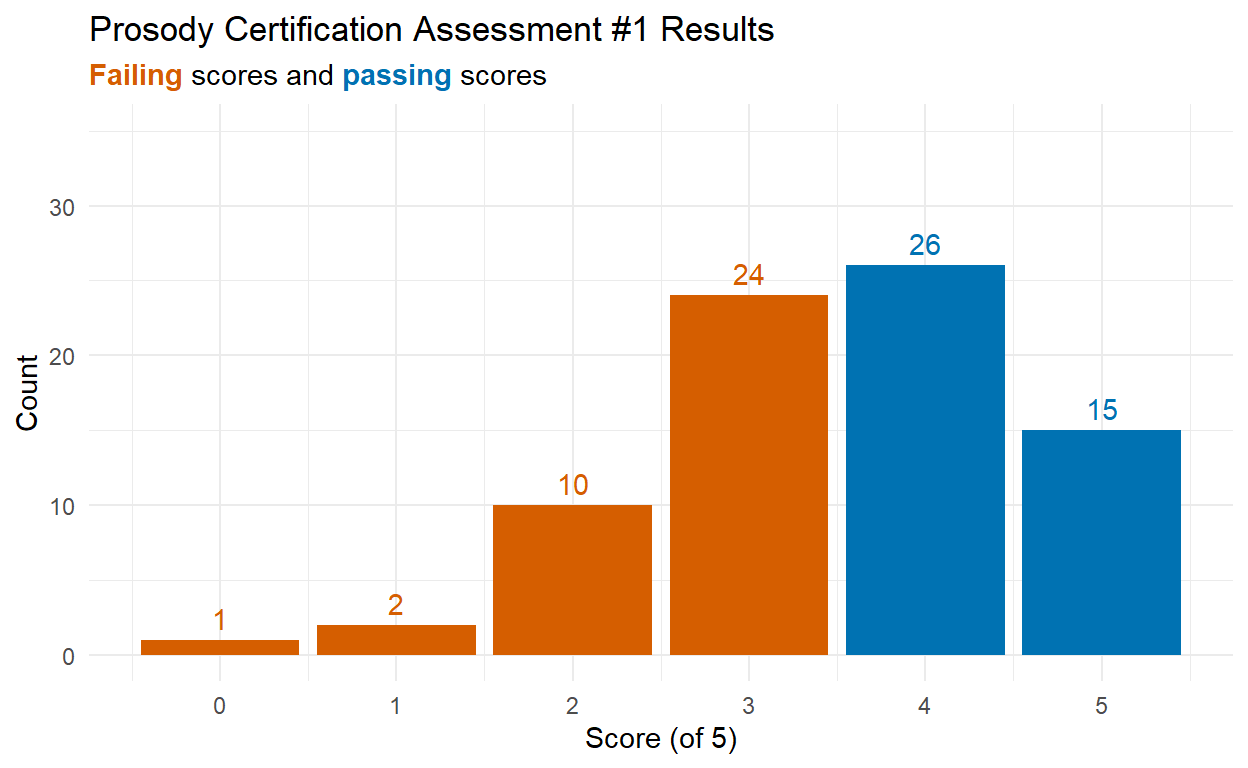
\includegraphics{annual_report_2021_files/figure-latex/unnamed-chunk-4-1.pdf}

\hypertarget{training-session-2}{%
\subsection{Training Session \#2}\label{training-session-2}}

One week later, participants again met with the research team for
Training Session \#2 (1.5 hours). Training Session \#2 consisted
primarily of a review of the five audio files from Prosody Certification
\#1. Participants were asked to listen to an audio file, with the
prosody score provided by the training facilitator, and to identify key
features that justified the score. After listening to an audio file,
they were asked to share in the Zoom platform's chat box prosody rubric
features (shown on the screen) of the reading that corresponded to the
score. The training facilitator read aloud and discussed the relevant
and important prosody score features, using the rubric to confirm scores
with participants. Participants were encouraged to ask questions if they
did not understand or disagreed with the prosody score. Each audio file
was played multiple times (three to six) to solidify the score and
rationale for the attendees. This process was repeated for each of the
five audio files.

Participants were then given an
\href{https://jnese.github.io/CORE-II_trainingwebsite/CORE_training_session2day2_FINAL.pdf}{introduction}
to and demonstration of the software that they would use to score the
audio files for prosody if they met certification. They were also
introduced to the
\href{https://jnese.github.io/CORE-II_trainingwebsite/index.html}{training
website}.

\hypertarget{prosody-rating-procedures}{%
\section{Prosody Rating Procedures}\label{prosody-rating-procedures}}

\hypertarget{prososy-raters-sample}{%
\subsection{Prososy Raters: Sample}\label{prososy-raters-sample}}

The final prosody sample included 57 prosody raters, 7 from each of FL
and IL, 4 from each of OR, 3 from each of IN, KS, NV and OH, 2 from each
of GA, ID, KY, MI, NC, UT and VA, and 1 from each of AL, AZ, CA, CO, LA,
MT, NM, NY, PA, SC, TN, TX and WA. Nearly all (55) raters were female, 1
was non-binary, and 1 chose not to response.

\hypertarget{highest-degree-earned}{%
\paragraph{Highest Degree Earned}\label{highest-degree-earned}}

Among the prosody raters, 32 (56\%) earned a Masters in education, 19
(33\%) earned a Bachelor, 2 (4\%) earned a Masters in another field, 2
(4\%) earned an Associate, and 2 (4\%) earned a Doctorate.

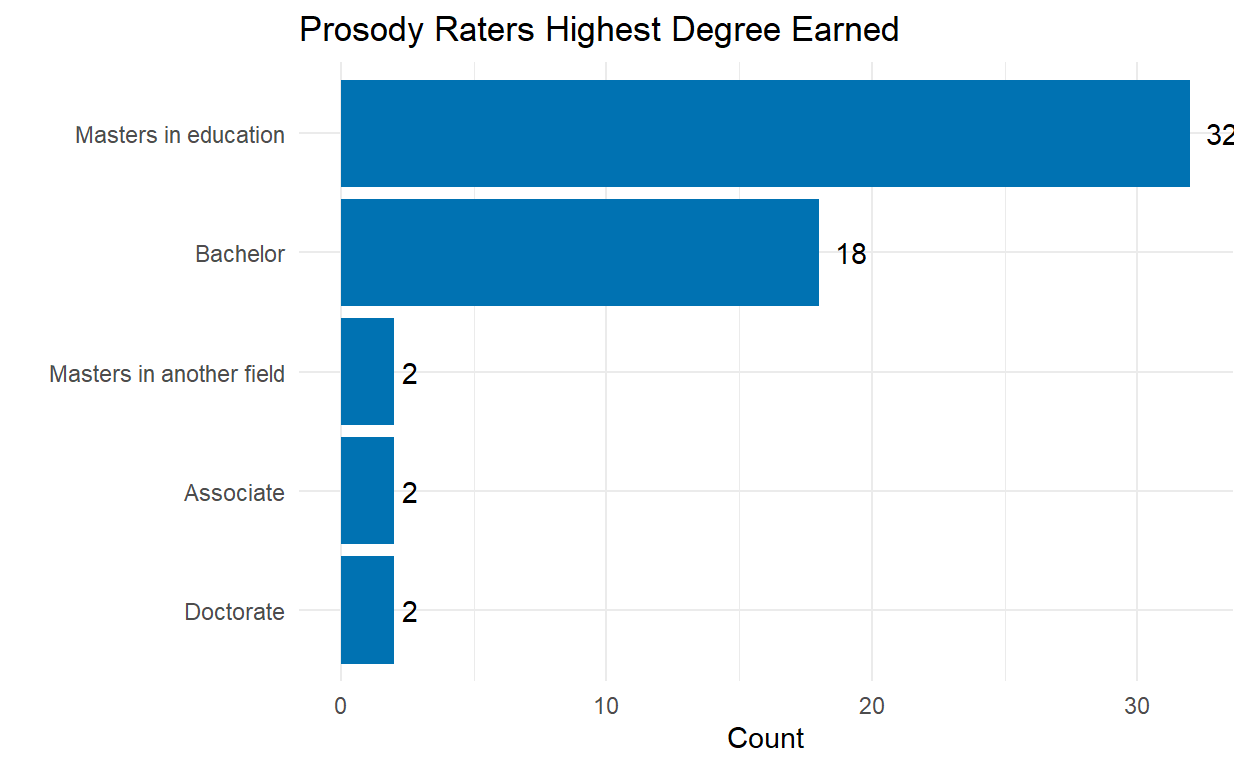
\includegraphics{annual_report_2021_files/figure-latex/degree_plot-1.pdf}

\hypertarget{professional-roles}{%
\paragraph{Professional Roles}\label{professional-roles}}

The professional roles of the raters were as follows:

\begin{itemize}
\item
  17 (30\%) were special education teachers
\item
  13 (23\%) were general education teachers
\item
  10 (18\%) were reading/literacy specialists
\item
  9 (16\%) reported as ``other''

  \begin{itemize}
  \tightlist
  \item
    (i.e., dyslexia program specialist; literacy tutor/data
    analyst/testing coordinator; project consultant supporting literacy,
    behavior and MTSS; RTI coordinator/interventionist; RTI specialist;
    MTSS lead; EC compliance case manager; Master's student; and
    undergraduate student studying elementary education)
  \end{itemize}
\item
  3 (5\%) reported as ``school psychologist \textbar{} social worker
  \textbar{} counselor \textbar{} behavior specialist \textbar{} etc.''
\item
  2 (4\%) reported as ``administrator \textbar{} principal \textbar{}
  district support''
\item
  2 (4\%) were retired, and reported their role as special educators
  before retirement
\item
  1 (19\%) an ``other content area specialist'' (i.e., ESOL)
\end{itemize}

\hypertarget{experience}{%
\paragraph{Experience}\label{experience}}

Nearly all of the prosody raters (\emph{n} = 48, 84\%) worked at the
elementary school level, 4 (7\%) worked at the middle school level, 2
(4\%) worked at the high school level, 1 (2\%) worked at the elementary
and middle levels, 1 (2\%) worked at all three levels, and 1 (2\%)
worked with adults.

The average years experience as an educator was 14 years (\emph{SD} =
9.9).

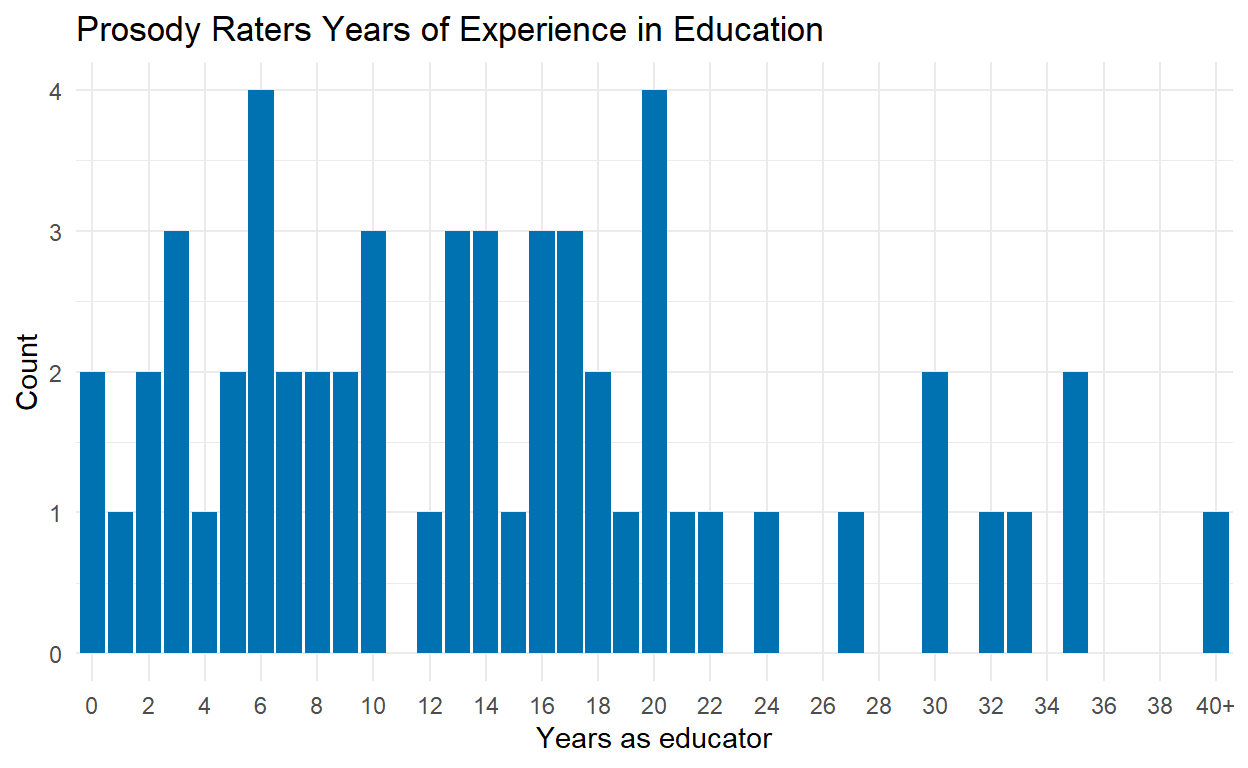
\includegraphics{annual_report_2021_files/figure-latex/experience_plot-1.pdf}

\hypertarget{prosody-raters-certification}{%
\subsection{Prosody Raters:
Certification}\label{prosody-raters-certification}}

All 57 prosody raters met the prosody certification criteria by scoring
at least 80\% on two Prosody Certification Assessments. Note that
Certification \#1 was taken after Training Session \#1, before the
Training was complete.

\captionsetup[table]{labelformat=empty,skip=1pt}
\begin{longtable}{lcclcl}
\caption*{
\large Prosody Certification Assessment Passing Rates\\ 
} \\ 
\toprule
 & n & Fail & Fail (\%) & Pass & Pass (\%) \\ 
\midrule
Certification \#1 & 57 & 26 & 46\% & 31 & 54\% \\ 
Certification \#2 & 55 & 12 & 22\% & 43 & 78\% \\ 
Certification \#3 & 31 & 2 & 6\% & 29 & 94\% \\ 
Certification \#4 & 6 & 2 & 33\% & 4 & 67\% \\ 
Certification \#5 & 2 & 0 & 0\% & 2 & 100\% \\ 
\bottomrule
\end{longtable}

Of the 57 people who took Certification \#1, 54\% passed by scoring 4 or
5; 78\% of the 55 people who took Certification \#2 passed; 94\% of the
31 people who took Certification \#3 passed; 67\% of the 6 people who
took Certification \#4 passed; and 100\% of the 2 people who took
Certification \#5 passed.

\begin{verbatim}
## Warning: Removed 4 rows containing missing values (position_stack).
\end{verbatim}

\begin{verbatim}
## Warning: Removed 4 rows containing missing values (geom_text).
\end{verbatim}

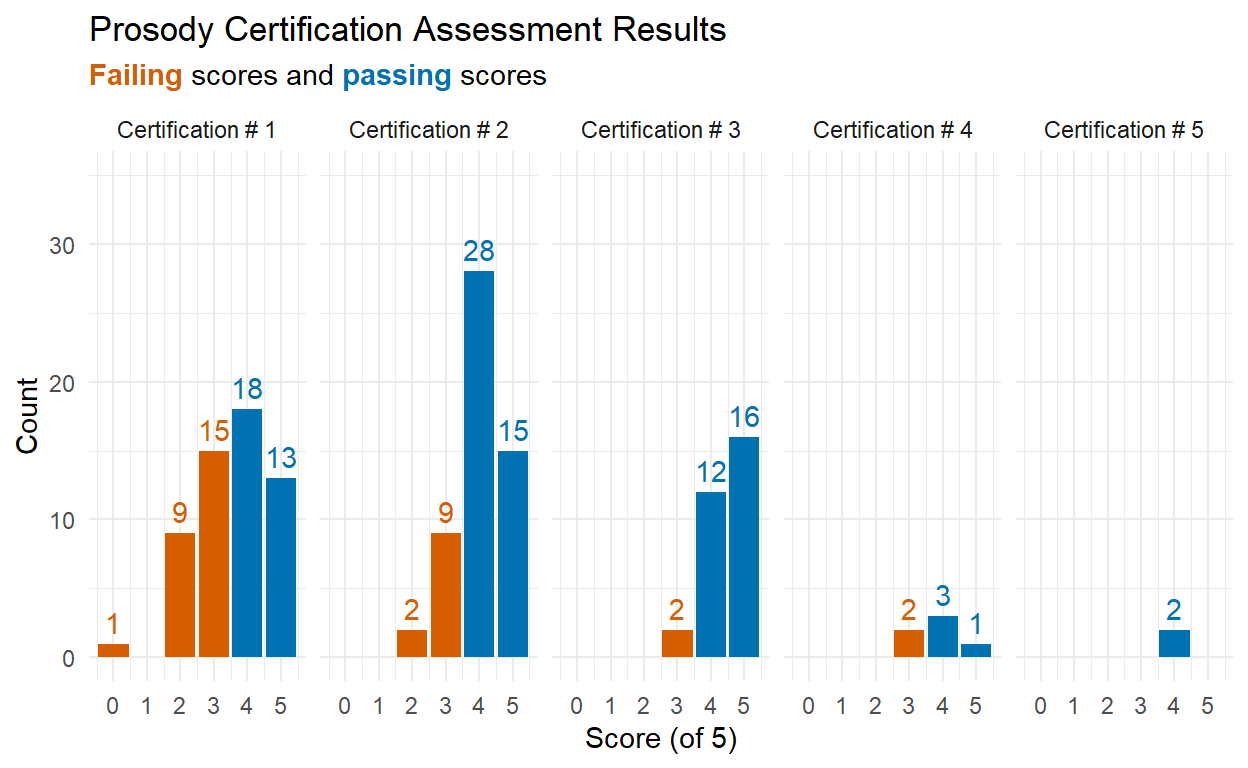
\includegraphics{annual_report_2021_files/figure-latex/raterscert_fig-1.pdf}

\begin{verbatim}
## Warning: Values are not uniquely identified; output will contain list-cols.
## * Use `values_fn = list` to suppress this warning.
## * Use `values_fn = length` to identify where the duplicates arise
## * Use `values_fn = {summary_fun}` to summarise duplicates
\end{verbatim}

\begin{verbatim}
## Warning: `cols` is now required when using unnest().
## Please use `cols = c(cert1_score, cert2_score, cert3_score, cert4_score, cert5_score)`
\end{verbatim}

The plot below shows which two Prosody Certification Assessments the
raters met prosody certification. Twenty-five raters (44\%) passed
Certification \#1 and Certification \#2, 17 (30\%) passed Certification
\#2 and Certification \#3, 6 (11\%) passed Certification \#1 and
Certification \#3, 4 (7\%) passed Certification \#3 and Certification
\#4, 1 (2\%) passed Certification \#2 and Certification \#5, and 1 (2\%)
passed Certification \#3 and Certification \#5.

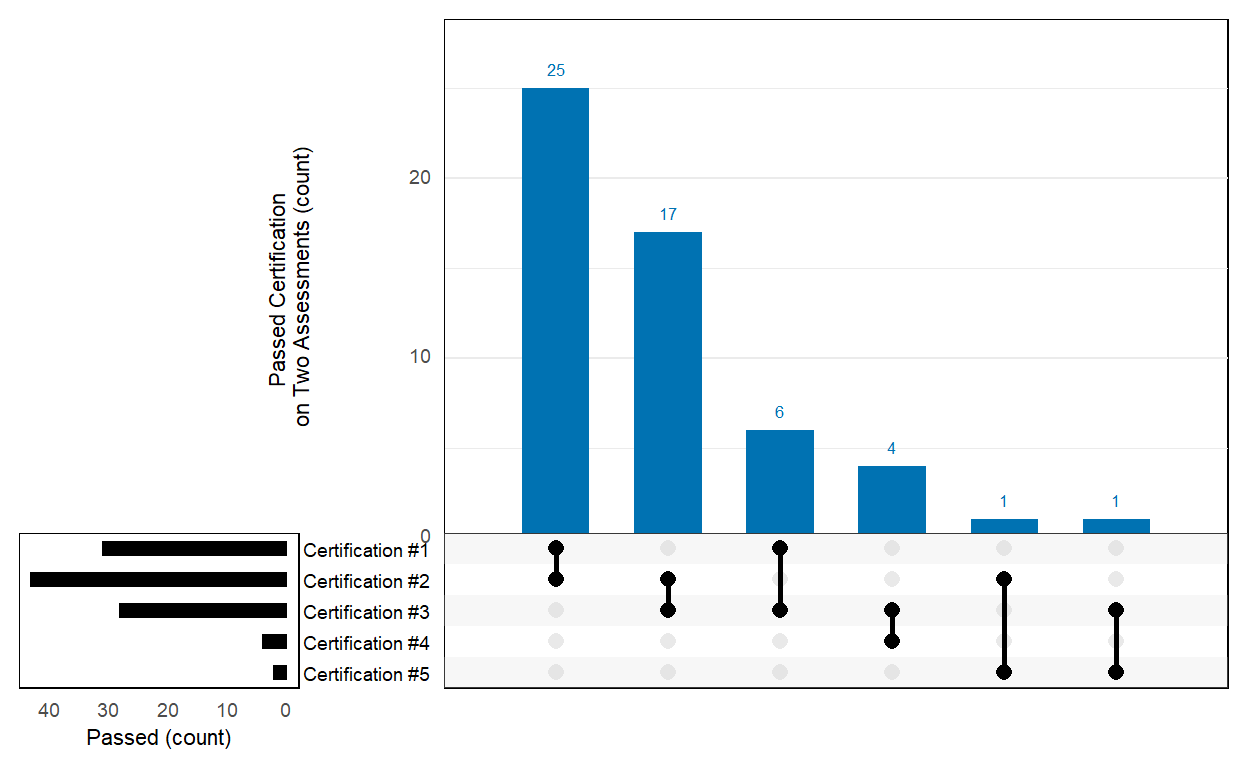
\includegraphics{annual_report_2021_files/figure-latex/upset_fig-1.pdf}

\hypertarget{prosody-ratings}{%
\subsection{Prosody Ratings}\label{prosody-ratings}}

The 57certified prosody raters created a profile on a project-designed
Moodle site. Raters each created their own log-in information for the
system. The system allowed raters to skip audio files, go back and
change scores, and complete the rating in multiple sessions, stopping
and re-starting as needed. In addition to the seven-point prosody scale
(1, 1.5, 2, 2.5, 3, 3.5, 4), raters were also given an option to note
``No audio available to score'' in case there was no audio (e.g., the
student was muted or advanced without reading) or the audio did not
allow the rater to confidently give a score (e.g., poor audio quality,
too much background noise, a very quiet reader).

The prosody raters were instructed to first complete a Prosody Review
containing four exemplar files, one at each prosody level (i.e, 1, 2, 3,
4), prior to rating their first set of audio files. The expectation was
set in training that raters must complete a minimum of 50 audio files;
there was no maximum. Upon completion of the first set of recordings,
raters emailed PI Nese to receive another set of recordings to rate.

In this manner, all 14,122 audio recordings were rated by two different
prosody raters from November 28, 2020 through February 8, 2021.

The median number of audio files scored by prosody raters was 182, with
a range from 50 to 865 (\emph{Mean} = 248, \emph{SD} = 203).

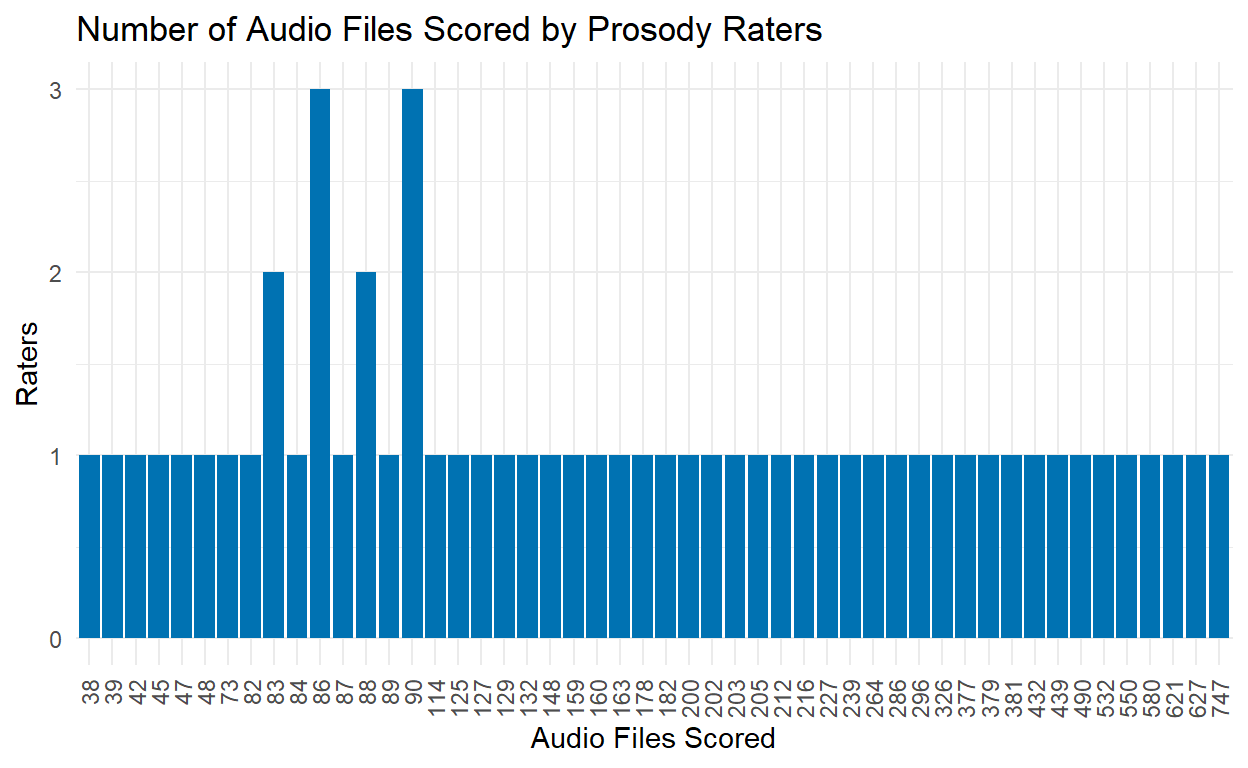
\includegraphics{annual_report_2021_files/figure-latex/ratefiles_fig-1.pdf}

\end{document}
